\subsection{Matriz AISI 304 y FEM}
\label{app:prototipo_A6}
La geometría del sólido de matriz coincide con la fuente anterior:
99\,mm exteriores, 102 canales 6\,mm, placa perforada 10\,mm, cubo y filetes reales.
Se reutilizan su geometría, material de diseño y ecuaciones de elasticidad;
no se reutiliza la solución FEM porque el apoyo inferior es ahora la cara
de la tuerca 1/2--13, sin la arandela inferior anterior.
Sus bordes circulares medidos tienen radio exterior 9,525\,mm. La zona común
plana de apoyo está limitada por el bore de matriz 6,5\,mm; su área es
$A_s=\pi(9,525^2-6,5^2)=152,291$ mm $^2$.
\begin{equation}
 p_{\min,\max}=F/A_s\mp Mr_o/I_s,\qquad
 I_s=\pi(r_o^4-r_i^4)/4.
\end{equation}
La presión máxima del equilibrio global es 6,028\,MPa
y la mínima 5,808\,MPa.
El contacto global permanece comprimido; ello no demuestra una distribución
unilateral completa ni la capacidad de fricción real de la unión.

\subsubsection*{Modelo y frontera}
Se importa el sólido STEP verificado en Gmsh/OCC. Se conservan placa,
agujeros, toros y filetes. En la cara plana inferior $y=26$ mm del STEP
individual se incorpora una curva de mallado de radio 9,525\,mm, sin editar
el STEP original. Se restringen los desplazamientos del anillo 6,5--9,525\,mm,
como apoyo rígido, bilateral y adherente: la retención y el torque deben
ser efectivamente provistos por la unión. No se fija la periferia.
Se emplean $E=200000$ MPa,$\nu=0,30$ y $R_{p0,2}=210$ MPa para 304 de
referencia H/P a 20gradosC~\cite{outokumpu_core_2026};$\nu$ es hipótesis
elástica. Los datos no certifican el material suministrado.

Las fuerzas de cada canal se recuperan con la integración corregida y
las holguras guardadas, sin nuevas iteraciones. Se aplican tracciones
equivalentes en paredes de canales, uniformes axialmente como hipótesis,
conservando $F_i$, fuerza total, torque y primer momento normal global.
La distribución positiva en paredes no representa un campo medido de
biomasa ni su presión radial interna. Se resuelve elasticidad 3D con
tetraedros lineales, CG/PyAMG y residuo relativo objetivo $10^{-9}$.
Se estudian los estados correlacionados de máximos de fuerza y torque,
no una combinación ficticia de ambos máximos.
El refinamiento adicional de frontera de 1\,mm permite hasta 1,25\,mm en el
interior y se aplica solo al caso gobernante 636, después de verificar
ambos casos 636 y 1291 hasta 1,25\,mm. El caso de fuerza máxima 1291 queda
por debajo del gobernante en esas mallas; no se repite innecesariamente.
\begin{center}\begin{tabular}{llllll}\toprule
Estado & $\theta$ [$^\circ$] & $F$ [N] & $T$ [N m] & $h_{\rm malla}$ [mm] & $\sigma_{VM}$ [MPa]\\\midrule
636 & 159,00 & 917,839 & 2,779984 & 1,00 & 38,710\\
1291 & 322,75 & 918,062 & 2,634896 & 1,25 & 31,057\\
\bottomrule\end{tabular}\end{center}
\begin{center}\begin{tabular}{llll}\toprule
$h_{\rm malla}$ [mm] & Tetraedros & Máx. $\sigma_{VM}$ [MPa] & Máx. $|u|$ [mm]\\\midrule
3,00 & 160132 & 32,906 & 0,01179\\
1,70 & 666308 & 35,785 & 0,01300\\
1,25 & 1595671 & 38,622 & 0,01352\\
1,00 & 3063761 & 38,710 & 0,01383\\
\bottomrule\end{tabular}\end{center}

El cambio de envolvente entre las dos últimas mallas es 0,23\% en tensión
y 2,31\% en desplazamiento, frente al criterio declarado 5\% en ambos.
La envolvente satisface el criterio numérico y el cribado elástico condicionado.
El máximo de la malla fina es 38,710\,MPa y el desplazamiento máximo
0,013833\,mm. El cociente de referencia $210/\sigma_{VM}=5,425$
se limita a estos casos y a las hipótesis de fijación/material. No se ha
resuelto contacto no lineal ni el historial FEM completo. La convergencia
de una envolvente no asegura la de cada pico secundario, cuyos cambios
se tabulan por separado. La máxima suma de reacciones axiales en sentido
de tracción de la malla fina es 0,122\,N:
es un diagnóstico de la restricción bilateral, no una fuerza definitiva
para dimensionar una tuerca. El peso de matriz,aproximadamente 3,97\,N,
se omite en el FEM frente a 918\,N y se incluye en la demanda del apoyo axial.
\begin{center}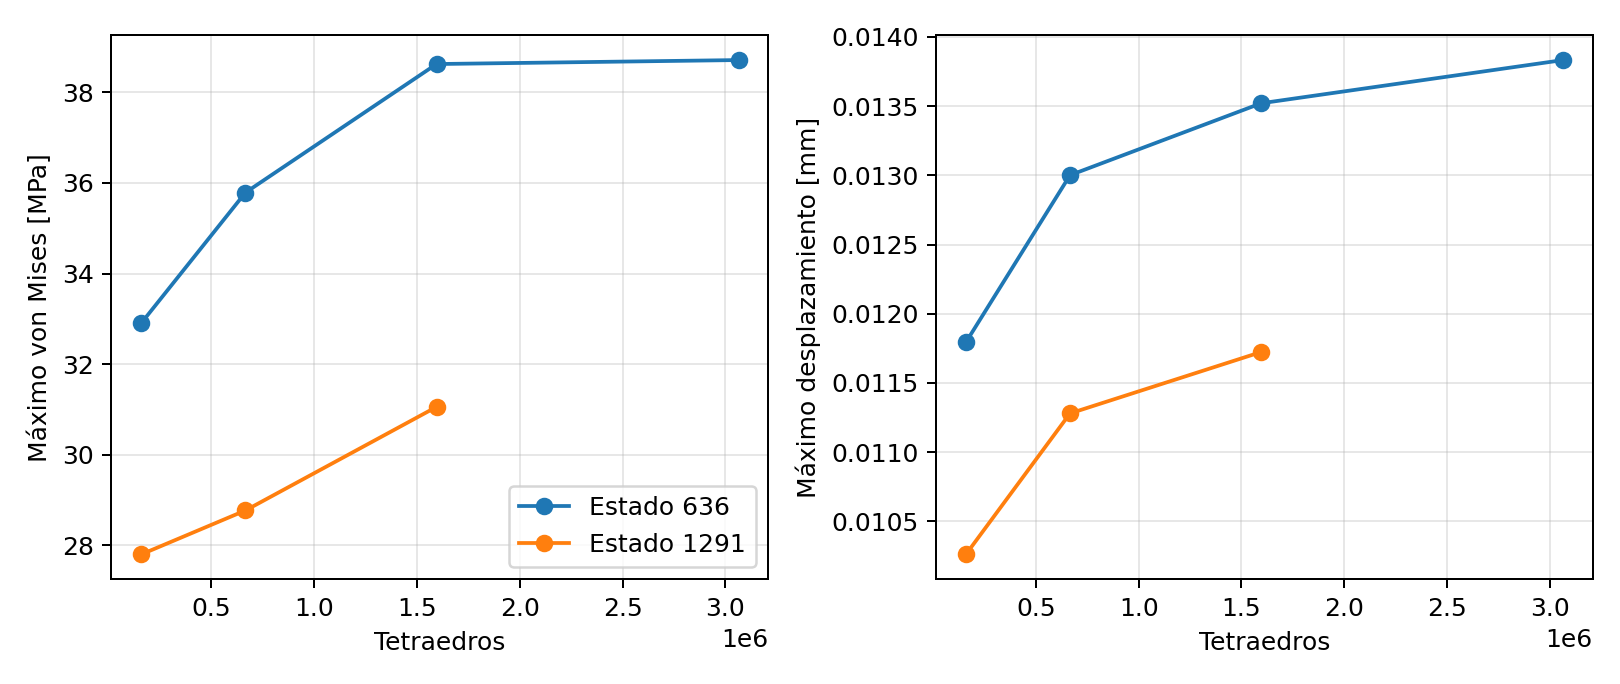
\includegraphics[width=.85\linewidth]{convergencia_fem.png}\end{center}
\begin{center}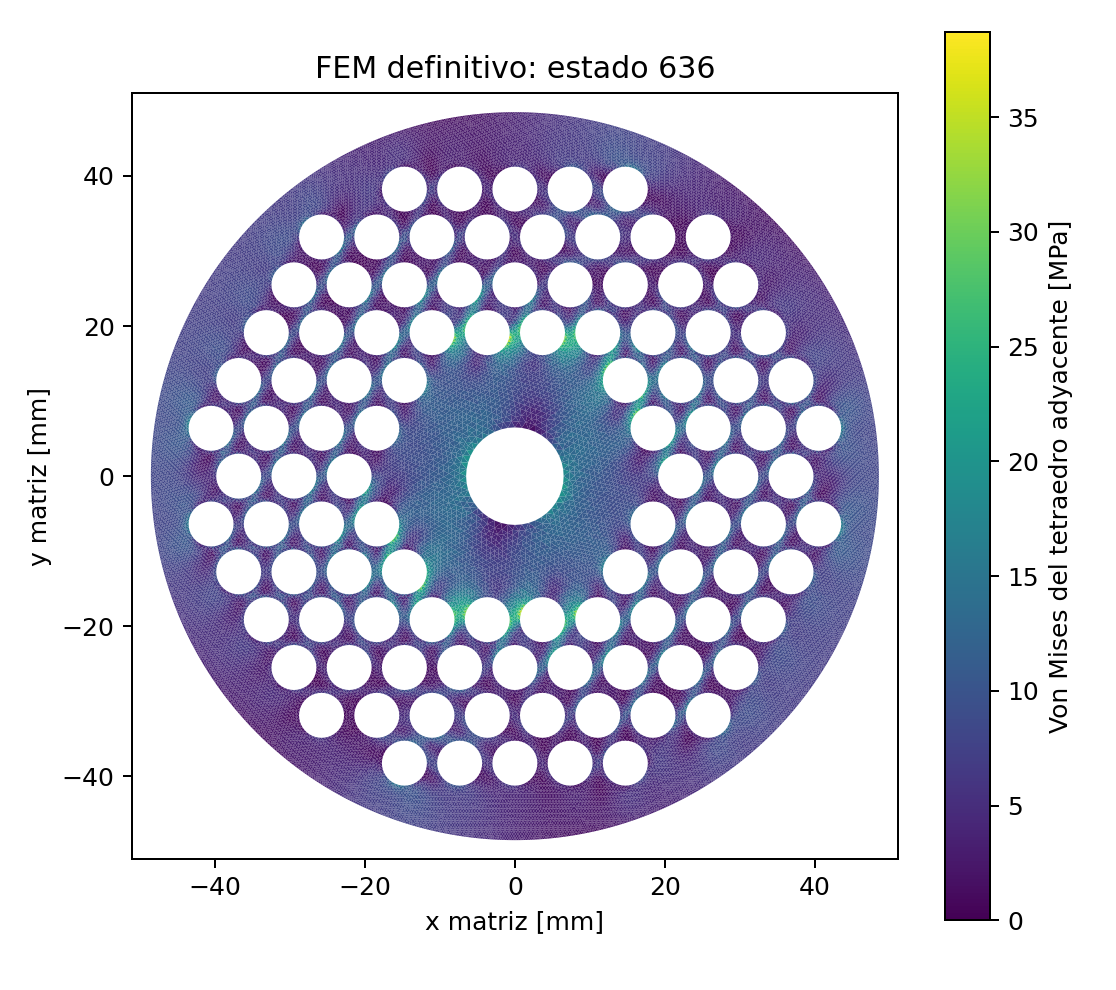
\includegraphics[width=.70\linewidth]{FEM_matriz.png}\end{center}
